\chapter{Kräfte, Phasenraum und Erhaltungssätze}

\lectureoverview{Ein Bewegungsgesetz muss mehr leisten, als bekannte physikalische Größen miteinander in Beziehung zu setzen. Es muss den Zustand eines Systems angeben, diesen Zustand von einem Zeitpunkt zum nächsten fortschreiben und erkennen lassen, welche Unterscheidungen und Größen die Bewegung überdauern. Wir nähern uns der Newtonschen Mechanik, indem wir zunächst ein plausibles, aber falsches Kraftgesetz prüfen, dann den Zustand von der Position auf den Phasenraum erweitern und schließlich die Erhaltung von Impuls und Energie herleiten.}

\section{Ein nützliches falsches Gesetz}

Die Bewegung im Alltag wird von Reibung beherrscht. Schiebt man einen schweren Gegenstand über den Boden, setzt er sich in Bewegung; hört man auf zu schieben, kommt er bald zum Stillstand. Ein stärkerer Schub führt im Allgemeinen zu einer höheren Geschwindigkeit, während ein schwererer Gegenstand kräftiger geschoben werden muss. In einer solchen Welt liegt die Annahme nahe, dass die Kraft unmittelbar die Geschwindigkeit erzeugt. Dies war die grundlegende Intuition hinter der aristotelischen Beschreibung der Bewegung.

Beim Schlittschuhlaufen macht man die fehlende Erfahrung. Ein Läufer braucht Kraft, um sich in Bewegung zu setzen, anzuhalten oder die Richtung zu ändern, aber nicht, um nach dem Anlaufen weiterzugleiten. Hätte Aristoteles auf nahezu reibungsfreiem Eis statt auf gewöhnlichem Boden gearbeitet, wäre der Fehler in der Kraft--Geschwindigkeit-Intuition viel schwerer zu übersehen gewesen.

Um den Fehler dieser Intuition offenzulegen, geben wir ihr eine präzise moderne Form. Wir schreiben die bewusst falsche Gleichung

\begin{equation}
  \mathbf F=m\mathbf v.
  \label{eq:aristotle-vector-law}
\end{equation}

Dies ist nicht Newtons Gesetz und sollte nicht als Physik auswendig gelernt werden. Ihr Wert liegt darin, dass sie der Diagnose dient: Sobald eine verbale Regel als Gleichung formuliert ist, können wir fragen, ob sie Bewegung vorhersagt und genügend Information bewahrt, um die Vergangenheit zu rekonstruieren. Der kurze Unterrichtsgesprächsbeitrag zum griechischen Wort für Kraft verweist auf \emph{dynamis}, die Wurzel, die auch in Wörtern wie Dynamo und Dynamik anklingt; für die Prüfung des Gesetzes selbst ist die Terminologie jedoch nebensächlich.

\begin{figure}[htbp]\centering
  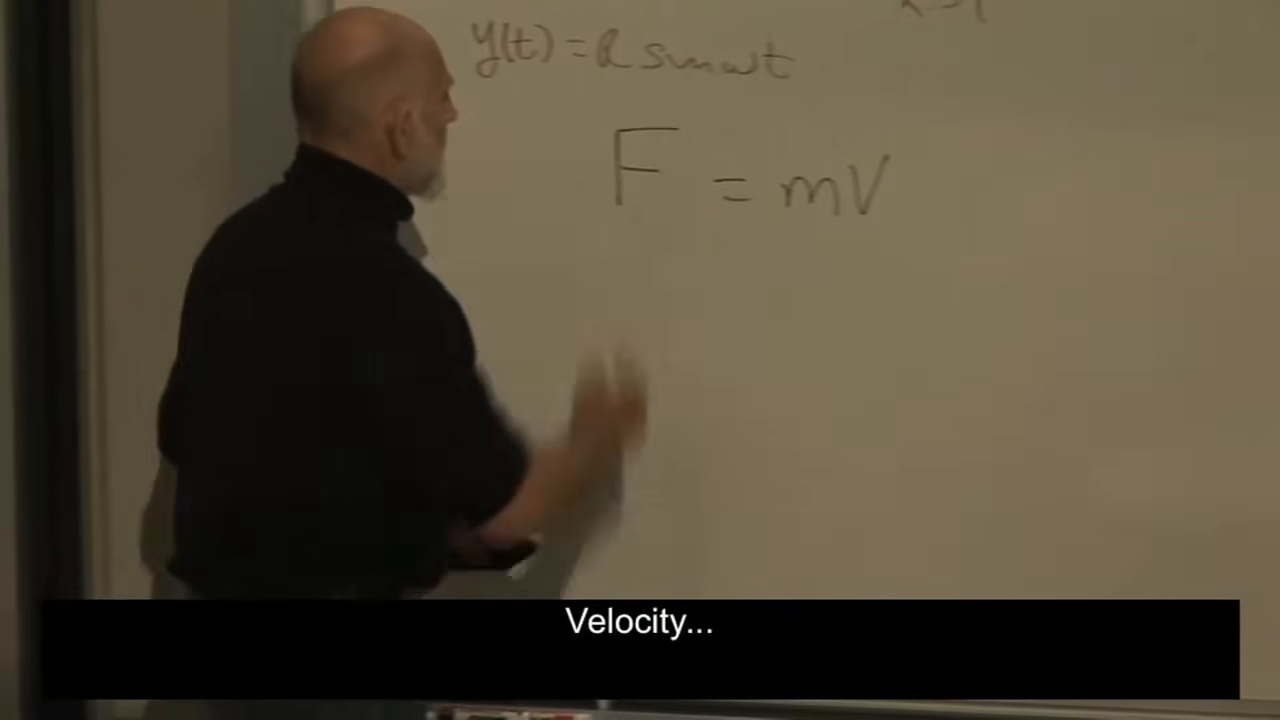
\includegraphics[width=0.82\textwidth]{lecture_02_figure_02.png}\caption{Das absichtlich falsche Kraft--Geschwindigkeit-Gesetz zur Prüfung von Vorhersagbarkeit und Umkehrbarkeit.}\lectureframe{00:04:51}\end{figure}

Beschränken wir die Bewegung auf eine Raumkoordinate. Da \(v=\dot x\) gilt, lautet das Gesetz

\begin{equation}
  F(t)=m\dot x(t).
  \label{eq:aristotle-1d}
\end{equation}

Teilen wir die Zeit nun in kurze Intervalle der Länge \(\delta\) ein. Während eines Intervalls gilt:

\begin{equation}
  \dot x(t)\simeq
  \frac{x(t+\delta)-x(t)}{\delta}.
  \label{eq:first-difference}
\end{equation}

Einsetzen in Gl.~\eqref{eq:aristotle-1d} ergibt

\begin{equation}
  x(t+\delta)
  =x(t)+\frac{\delta}{m}F(t).
  \label{eq:aristotle-update}
\end{equation}

Dies hat die Form einer echten Aktualisierungsregel. Sind die gegenwärtige Position und die Kraft bekannt, folgt daraus die Position zum nächsten stroboskopischen Zeitpunkt. Verschwindet die Kraft, ergibt Aristoteles’ Regel jedoch \(\dot x=0\): Der Gegenstand muss in Ruhe bleiben. Eine Bewegung ohne aufrechterhaltende Kraft ist von Anfang an ausgeschlossen.

\begin{figure}[htbp]\centering
  \includegraphics[width=0.84\textwidth]{lecture_02_figure_07.png}\caption{Die diskrete Aktualisierung nach Aristoteles mit einer rücktreibenden Kraft. Bei jedem Schritt wird die Auslenkung mit einem Faktor multipliziert, der geringfügig kleiner als eins ist.}\lectureframe{00:10:15}\end{figure}

\subsection{Eine Feder in der Mechanik des Aristoteles}

Betrachten wir ein Teilchen, das an einer Feder befestigt ist, deren Gleichgewichtslage bei \(x=0\) liegt. Eine Auslenkung erzeugt die rücktreibende Kraft

\begin{equation}
  F(x)=-kx,
  \qquad k>0.
  \label{eq:hooke-law}
\end{equation}

Setzen wir diese Kraft in Gl.~\eqref{eq:aristotle-update} ein, erhalten wir

\begin{equation}
  x(t+\delta)
  =\left(1-\frac{k\delta}{m}\right)x(t).
  \label{eq:aristotle-spring-update}
\end{equation}

Für hinreichend kleines \(\delta\) liegt der Faktor in der Klammer knapp unter eins. Bei jeder Aktualisierung wird die Auslenkung daher um denselben Anteil verringert:

\begin{equation}
  x_n=\left(1-\frac{k\delta}{m}\right)^n x_0.
  \label{eq:aristotle-geometric-decay}
\end{equation}

Die kontinuierliche Gleichung und ihre Lösung lauten

\begin{align}
  m\dot x&=-kx,
  \label{eq:aristotle-spring-continuous}\\
  x(t)&=x(0)e^{-kt/m}.
  \label{eq:aristotle-spring-solution}
\end{align}

Die Feder führt keine Schwingung aus. Aus jeder Auslenkung freigegeben, nähert sie sich exponentiell dem Ursprung und bewegt sich dabei immer langsamer.

\begin{figure}[htbp]\centering
  \includegraphics[width=0.84\textwidth]{lecture_02_figure_08.png}\caption{Die exponentielle Lösung der aristotelischen Federgleichung. Die Auslenkung klingt ab, statt zu schwingen.}\lectureframe{00:12:02}\end{figure}

Die Zukunft lässt sich leicht vorhersagen: Jede anfängliche Auslenkung nähert sich derselben Ruhelage. Mit der Vergangenheit ist es anders. Angenommen, das Teilchen wird sehr nahe am Ursprung und nur mit endlicher Genauigkeit beobachtet. Es könnte bei einer von vielen verschiedenen Auslenkungen begonnen haben, denn ihre exponentiell kleinen Reste liegen schließlich alle innerhalb derselben Messtoleranz. Bei perfekter mathematischer Genauigkeit lässt sich Gl.~\eqref{eq:aristotle-spring-solution} rückwärts durchlaufen, doch praktische Unterschiede zwischen den Vorgeschichten werden nach und nach ausgelöscht. Vom Standpunkt einer umkehrbaren fundamentalen Dynamik aus ist das Gesetz daher verdächtig.

Das bedeutet nicht, dass Aristoteles irrational war. Die von ihm beschriebene, reibungsdominierte Bewegung ist tatsächlich dissipativ. Der Fehler bestand darin, dieses effektive Verhalten zu einem fundamentalen Gesetz zu erheben. Reibung ist selbst eine Kraft, die aus komplizierten mikroskopischen Wechselwirkungen entsteht. Schiebt eine Hand einen Gegenstand ungefähr mit gleichbleibender Geschwindigkeit, gleicht die ausgeübte Kraft die Reibung aus; sie erzeugt nicht die Geschwindigkeit als solche.

\section{Newtons Gesetz und seine physikalische Bedeutung}

Die Newtonsche Korrektur lautet: Eine Kraft ändert die Bewegung:

\begin{equation}
  \mathbf F=m\mathbf a=m\ddot{\mathbf x}.
  \label{eq:newton-second-law}
\end{equation}

Bevor wir dies als Entwicklungsgleichung auffassen, müssen wir zwei scheinbare Zirkelschlüsse auflösen. Der erste betrifft Bezugssysteme. Oft hört man, Newtons Gesetze gälten in Inertialsystemen und ein Inertialsystem sei eines, in dem Newtons Gesetze gelten. Die physikalische Aussage ist nicht diese zirkuläre Definition. Sie ist die empirische Behauptung, dass \emph{es} Bezugssysteme gibt, die durch geeignete Maßstäbe und Uhren beschrieben werden und in denen Newtons Gesetze ihre einfache Form annehmen. Bezugssysteme, die sich relativ zu ihnen beschleunigen oder drehen, erfordern zusätzliche Scheinkräfte. Wie sich die Gleichungen in diesen anderen Bezugssystemen transformieren, lässt sich später herleiten.

Der zweite Zirkelschluss betrifft Kraft und Masse. Definiert man die Kraft als Masse mal Beschleunigung und die Masse als Kraft geteilt durch Beschleunigung, scheint die Gleichung leer zu sein. Ein operationales Experiment trennt die Definitionen vom Gesetz. Man vergleicht einen Gegenstand mit einem Normkilogramm, indem man beide ins Gleichgewicht bringt, und befestigt den Gegenstand dann in einem ansonsten kraftfreien Raum an einer Federwaage. Eine feste kleine Dehnung der Feder wird als eine Krafteinheit definiert. Zwei identische Federn, die jeweils um denselben Betrag gedehnt werden, liefern zwei Krafteinheiten und erzeugen die doppelte Beschleunigung. Es ist sicherer, eine zweite Feder hinzuzufügen, als eine einzelne Feder doppelt so weit zu dehnen, denn eine reale Feder wird schließlich nichtlinear oder reißt. Lässt man eine Feder unverändert und verbindet sie mit zwei gleichen Massen, beträgt die Beschleunigung die Hälfte; bei drei gleichen Massen beträgt sie ein Drittel.

\begin{figure}[htbp]\centering
  \includegraphics[width=0.84\textwidth]{lecture_02_figure_09.png}\caption{Das Gedankenexperiment mit der Federwaage dient dazu, gleiche Krafteinheiten zu definieren und die Proportionalität der Beschleunigung zur Kraft zu prüfen.}\lectureframe{00:22:45}\end{figure}

Diese Vergleiche verleihen folgender Beziehung empirischen Gehalt:

\begin{equation}
  a\propto F,
  \qquad
  a\propto\frac{1}{m},
  \qquad
  F=ma.
  \label{eq:force-mass-scaling}
\end{equation}

Das Wort \emph{Teilchen} verwenden wir für jeden kleinen Gegenstand, dessen innere Struktur keine Rolle spielt, nicht nur für ein Elementarteilchen.

\subsection{Warum die Position allein kein Zustand ist}

Prüfen wir Newtons Gleichung nun mit derselben stroboskopischen Methode. Der zentrierte Differenzenquotient für die Beschleunigung lautet

\begin{equation}
  \ddot x(t)\simeq
  \frac{x(t+\delta)-2x(t)+x(t-\delta)}{\delta^2}.
  \label{eq:second-difference}
\end{equation}

Daraus folgt aus Newtons Gleichung

\begin{equation}
  x(t+\delta)
  =2x(t)-x(t-\delta)+\frac{\delta^2}{m}F(t).
  \label{eq:newton-position-update}
\end{equation}

Die nächste Position lässt sich nicht allein aus \(x(t)\) bestimmen. Wir benötigen auch die vorherige Position \(x(t-\delta)\) oder gleichbedeutend die Geschwindigkeit zum gegenwärtigen Zeitpunkt. Zunächst scheint Newtons Gleichung dadurch weniger vorhersagekräftig als diejenige von Aristoteles. Die richtige Schlussfolgerung lautet vielmehr, dass die Position allein den Zustand nicht vollständig beschrieb. Alles Relevante zu einem Zeitpunkt zu kennen bedeutet, genügend Daten zu kennen, um die anschließende Bewegung zu bestimmen. Für ein Newtonsches Teilchen sind das Position und Geschwindigkeit.

\section{Impuls und Phasenraum}

Wir führen den Impuls ein durch

\begin{equation}
  \mathbf p=m\mathbf v=m\dot{\mathbf x}.
  \label{eq:momentum-definition}
\end{equation}

Die Masse eines festgelegten Newtonschen Systems wird als konstant angenommen. Ein Gegenstand kann ein Teil verlieren, wie ein Stift seine Kappe, doch dann hat sich der beschriebene Gegenstand geändert; das gewählte abgeschlossene System behält weiterhin seine konstante Gesamtmasse. Bei konstantem \(m\) wird Newtons zweites Gesetz zu

\begin{equation}
  \mathbf F=\dot{\mathbf p}.
  \label{eq:newton-momentum-form}
\end{equation}

\begin{figure}[htbp]\centering
  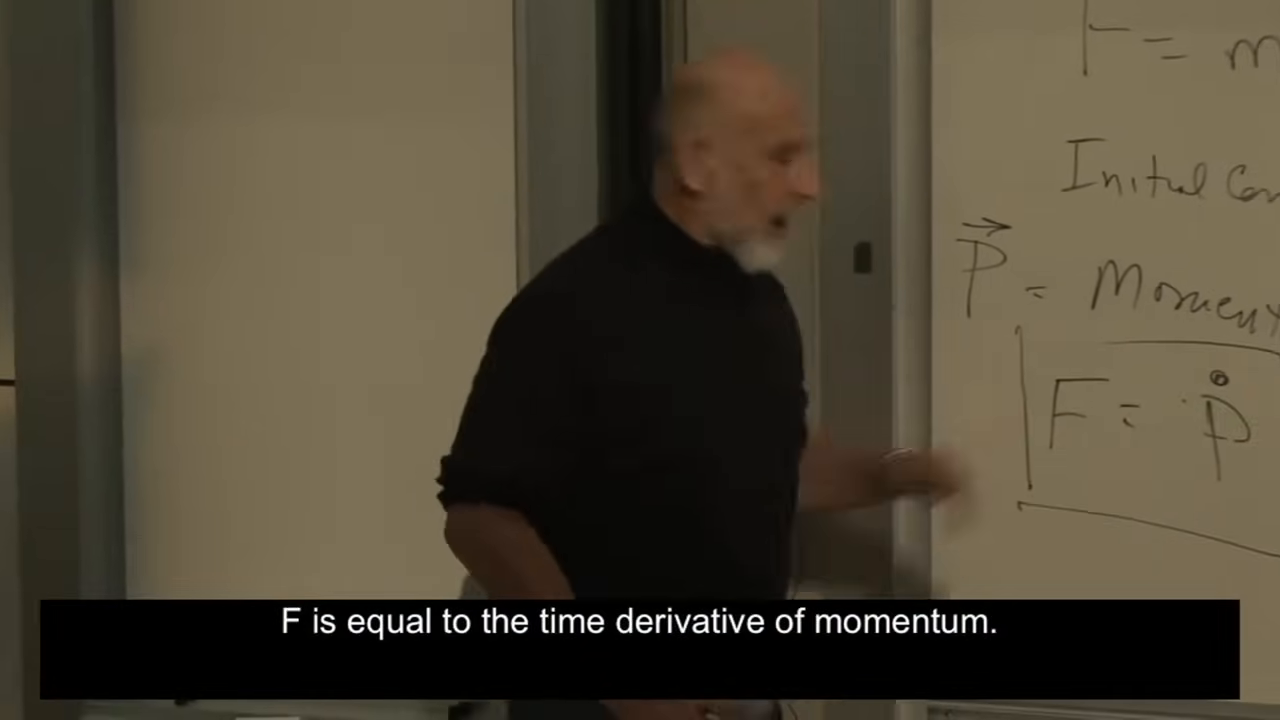
\includegraphics[width=0.82\textwidth]{lecture_02_figure_03.png}\caption{Newtons Gesetz als zeitliche Ableitung des Impulses geschrieben.}\lectureframe{00:32:35}\end{figure}

Für eine Koordinate lässt sich die Newtonsche Bewegung nun durch zwei Differentialgleichungen erster Ordnung für zwei unabhängige Zustandsvariablen beschreiben:

\begin{align}
  \dot p&=F(x,t),
  \label{eq:first-order-p}\\
  \dot x&=\frac{p}{m}.
  \label{eq:first-order-x}
\end{align}

Die eine Gleichung gibt an, wie die Kraft den Impuls ändert; die andere, wie der Impuls die Position ändert. Ihre diskrete Form erster Ordnung lautet

\begin{align}
  p(t+\delta)&=p(t)+\delta F(x(t),t)+O(\delta^2),
  \label{eq:momentum-discrete}\\
  x(t+\delta)&=x(t)+\frac{\delta}{m}p(t)+O(\delta^2).
  \label{eq:position-discrete}
\end{align}

Sind \(x(t)\) und \(p(t)\) gegeben, bestimmen diese Gleichungen das nächste Wertepaar, das dann als Eingabe für den nächsten Schritt dient. Die Bahn entsteht durch wiederholte Aktualisierungen.

\begin{figure}[htbp]\centering
  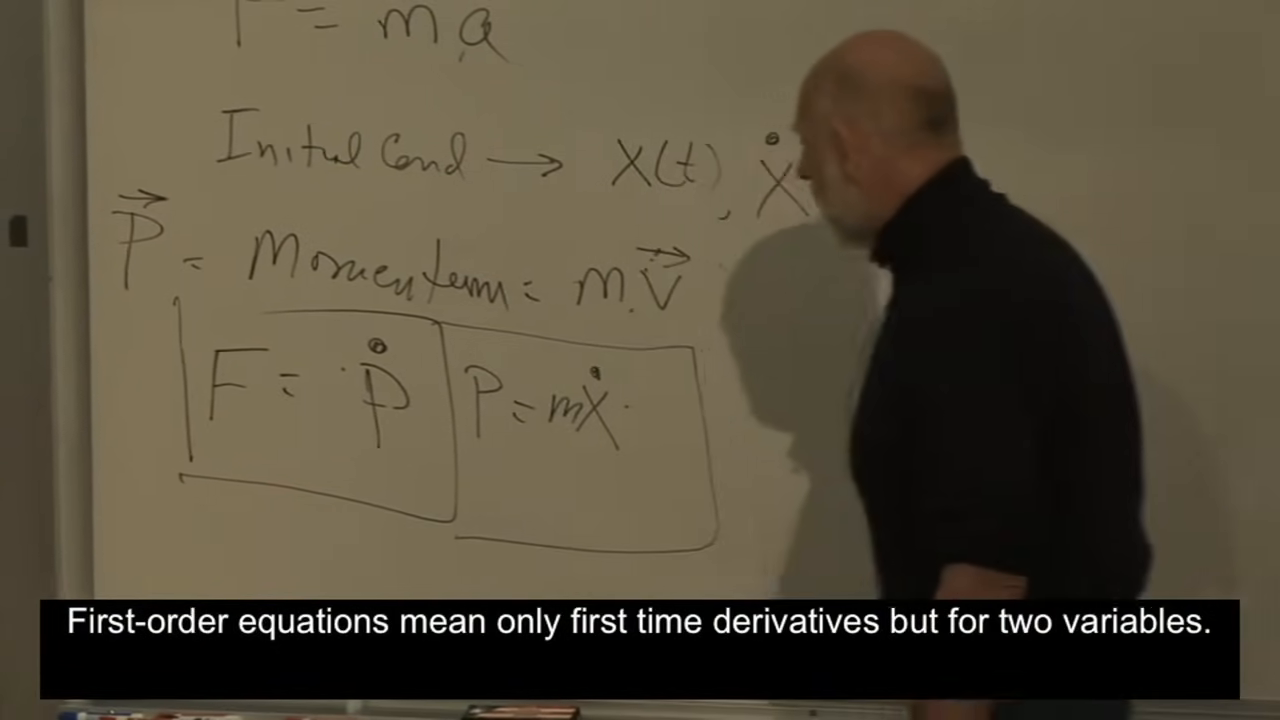
\includegraphics[width=0.84\textwidth]{lecture_02_figure_04.png}\caption{Die beiden Differentialgleichungen erster Ordnung und die zugehörigen Anfangsdaten. Position und Impuls legen gemeinsam den Zustand fest.}\lectureframe{00:35:47}\end{figure}

Der Raum aller Paare \((x,p)\) heißt \emph{Phasenraum}. Für ein Teilchen, das sich in drei Dimensionen bewegt, hat er sechs Koordinaten:

\begin{equation}
  (x,y,z,p_x,p_y,p_z).
  \label{eq:one-particle-phase-space}
\end{equation}

Der Phasenraum ist der Raum vollständiger Anfangsbedingungen. Der Konfigurationsraum erfasst nur Positionen; der Phasenraum enthält genau die Daten, die das Bewegungsgesetz benötigt.

\begin{classroomqa}\audiencequestion{Wird die Aktualisierung komplizierter, wenn die Kraft eine Funktion der Position statt eine bekannte Funktion der Zeit ist?\lecturetimestamp{00:36:27--00:37:07}}\lecturerresponse{Die Gleichungen bleiben vorhersagekräftig. Sobald \(x\) und \(p\) bekannt sind, ist auch der Wert \(F(x)\) bekannt. Gleichung~\eqref{eq:first-order-p} schreitet mit \(p\) fort, Gl.~\eqref{eq:first-order-x} mit \(x\), und das aktualisierte Wertepaar kann erneut verwendet werden.}\end{classroomqa}

\section{Die Newtonsche Feder}

Kehren wir zur Feder zurück, um die beiden Gesetze unter denselben physikalischen Bedingungen zu vergleichen. Nach Newton gilt

\begin{equation}
  m\ddot x=-kx.
  \label{eq:newton-spring}
\end{equation}

Setzen wir vorübergehend \(m=k=1\), um die Konstanten zu entfernen. Dann gilt

\begin{equation}
  \ddot x=-x.
  \label{eq:normalized-oscillator}
\end{equation}

Anders als die Exponentialfunktion kehren Sinus und Kosinus nach zweimaligem Ableiten zu ihrem Negativen zurück. Die allgemeine Lösung lässt sich schreiben als

\begin{align}
  x(t)&=C\cos(t-t_0),
  \label{eq:oscillator-x}\\
  p(t)=\dot x(t)&=-C\sin(t-t_0).
  \label{eq:oscillator-p}
\end{align}

Die beiden Konstanten enthalten die zwei Angaben über den Anfangszustand. Die Amplitude \(C\) gibt die maximale Auslenkung an, während \(t_0\) die Phase festlegt, hier so gewählt, dass die Geschwindigkeit bei \(t=t_0\) null ist. An den Endpunkten kommt das Teilchen nur für einen Augenblick zum Stillstand. Dann kehrt es durch den Ursprung zurück, wo seine Geschwindigkeit und sein Impuls am größten sind, und schwingt weiter.

Quadrieren wir die Gl.~\eqref{eq:oscillator-x} und \eqref{eq:oscillator-p}, erhalten wir

\begin{equation}
  x^2+p^2=C^2.
  \label{eq:oscillator-phase-circle}
\end{equation}

Der Punkt im Phasenraum bewegt sich somit auf einem Kreis mit dem Radius \(C\). Verschiedene Anfangsamplituden ergeben verschiedene Kreise; eine Änderung von \(t_0\) wählt einen anderen Ausgangspunkt auf demselben Kreis. In diesen normierten Einheiten wird jeder Kreis mit derselben Periodendauer \(2\pi\) durchlaufen, unabhängig von der Amplitude.

\begin{figure}[htbp]\centering
  \includegraphics[width=0.84\textwidth]{lecture_02_figure_10.png}\caption{Die Oszillatorlösung und ihre Kreisbahn in der \((x,p)\)-Phasenebene.}\lectureframe{00:43:20}\end{figure}

\begin{figure}[htbp]\centering
  \begin{tikzpicture}[scale=1.05,>=Latex]
    \draw[->] (-2.6,0) -- (2.75,0) node[right] {$x$};
    \draw[->] (0,-2.4) -- (0,2.55) node[above] {$p$};
    \draw[blue!65!black,thick] (0,0) circle (1.85);
    \draw[->,blue!65!black,thick]
      (1.60,0.93) arc[start angle=30,end angle=72,radius=1.85];
    \fill[red!65!black] (1.60,0.93) circle (2pt);
    \draw[dashed] (0,0) -- (1.60,0.93)
      node[midway,below right] {$C$};
    \node[align=left] at (-1.55,1.85)
      {$x=C\cos(t-t_0)$\\$p=-C\sin(t-t_0)$};
  \end{tikzpicture}\caption{Eine Phasenraumtrajektorie bewahrt sowohl Position als auch Impuls. Ihr Radius kennzeichnet die Bewegung, während der Winkel gleichförmig mit der Zeit zunimmt.}\label{fig:oscillator-phase-space}\end{figure}

Die Projektion auf die horizontale Achse ergibt die bekannte Hin- und Herbewegung von \(x\); die Projektion auf die vertikale Achse ergibt die Schwingung von \(p\). Anders als bei der aristotelischen Feder fallen verschiedene Kreise niemals zusammen. Kennt man einen Punkt im Phasenraum, so sind sowohl seine Zukunft als auch seine Vergangenheit bestimmt.

Für allgemeines \(m\) und \(k\) lautet die Kreisfrequenz

\begin{equation}
  \omega=\sqrt{\frac{k}{m}},
  \qquad
  x(t)=C\cos\bigl(\omega(t-t_0)\bigr),
  \label{eq:general-oscillator-frequency}
\end{equation}

und die Phasenraumtrajektorie wird in der nicht skalierten \((x,p)\)-Ebene zu einer Ellipse. Das Kreismodell ist die praktische Normierung \(m=k=1\), die in der Vorlesung verwendet wird.

\begin{classroomqa}\audiencequestion{Ginge die Vorhersagbarkeit verloren, wenn in der Oszillatorgleichung die zweite Ableitung durch eine erste Ableitung ersetzt würde?\lecturetimestamp{00:45:23--00:46:04}}\lecturerresponse{Nein. Auch eine Differentialgleichung erster Ordnung kann die Bewegung ausgehend von geeigneten Anfangsdaten vorhersagen. Die weitergehende Frage ist, ob ihr Fluss Unterschiede ausreichend bewahrt, um umkehrbar zu sein; der entsprechende allgemeine Satz wird erst behandelt, wenn die nötigen mathematischen Mittel bereitstehen.}\end{classroomqa}

\section{Zeitumkehr}

Das Oszillatorbild macht die Umkehrbarkeit anschaulich, doch die Gleichungen lassen sich auch direkt prüfen. Führen wir eine umgekehrte Zeitkoordinate ein:

\begin{equation}
  T=-t.
  \label{eq:reverse-time}
\end{equation}

Dann gilt

\begin{equation}
  \frac{d}{dt}=-\frac{d}{dT},
  \qquad
  \frac{d^2}{dt^2}=\frac{d^2}{dT^2}.
  \label{eq:time-derivative-parity}
\end{equation}

Bei einer Zeitumkehr wechselt eine erste Ableitung ihr Vorzeichen, eine zweite Ableitung dagegen nicht. Folglich behält die autonome aristotelische Gleichung

\begin{equation}
  m\dot x=F(x)
  \label{eq:aristotle-time-reversal}
\end{equation}

ihre Form nicht bei, wenn ein Film rückwärts abgespielt wird. Aus einer abklingenden Feder würde eine Feder, die sich spontan aus dem Gleichgewicht entfernt. Dagegen bleibt

\begin{equation}
  m\ddot x=F(x)
  \label{eq:newton-time-reversal}
\end{equation}

unverändert. Bei der Umkehr eines Newtonschen Films kehrt sich die Geschwindigkeit um, die Beschleunigung bleibt jedoch unverändert; deshalb ist der rückwärts laufende Film ebenfalls eine zulässige Lösung.

\begin{figure}[htbp]\centering
  \includegraphics[width=0.84\textwidth]{lecture_02_figure_11.png}\caption{Vergleich an der Tafel unter \(t\mapsto -t\): Erste Ableitungen wechseln ihr Vorzeichen, zweite Ableitungen dagegen nicht.}\lectureframe{00:50:45}\end{figure}

\begin{classroomqa}\audiencequestion{Warum sollte Umkehrbarkeit als allgemeine Voraussetzung der Physik gelten?\lecturetimestamp{00:46:16--00:48:26}}\lecturerresponse{Sie wird geprüft, nicht durch Definition garantiert. Wir untersuchen erfolgreiche Gesetze, erkennen gemeinsame Merkmale in Experimenten und erheben diese Merkmale zu Prinzipien. Die tiefere logische Ordnung verläuft in die entgegengesetzte Richtung: Die Quantenfeldtheorie ist fundamentaler, und die Newtonsche Mechanik ergibt sich durch Näherungen wie langsame Bewegung und große Massen. Ein Lehrgang muss sich von einfacheren Gesetzen ausgehend aufbauen; deshalb führen wir die Umkehrbarkeit jetzt als Prinzip ein, dessen Geltungsbereich später geprüft wird.}\end{classroomqa}

\begin{classroomqa}\audiencequestion{War die Umkehrbarkeit selbst ein Problem, das Newton bewusst erkannte?\lecturetimestamp{00:48:28--00:49:02}}\lecturerresponse{Die historische Antwort ist ungewiss. Newton verstand sicherlich das Trägheitsprinzip: Eine Kraft ist nötig, um einen Bewegungszustand zu ändern, nicht um eine gleichförmige Bewegung aufrechtzuerhalten. Ob er diese Einsicht ausdrücklich im Hinblick auf Umkehrbarkeit formulierte, ist eine davon getrennte historische Frage.}\end{classroomqa}

\section{Zyklen und Erhaltungsgrößen}

Die Kreise im Phasenraum legen den nächsten Gedanken nahe. Eine Trajektorie bleibt auf einem Kreis und springt niemals auf einen anderen. Der Kreis lässt sich daher durch eine Zahl kennzeichnen, die während der Bewegung konstant bleibt. Für den normierten Oszillator ist diese Zahl

\begin{equation}
  C^2=x^2+p^2.
  \label{eq:cycle-label}
\end{equation}

Bis auf einen Faktor von ein halb ist dies die Energie des Oszillators. Größere Kreise haben eine größere Energie; eine Änderung der Anfangsphase ändert sie nicht. Wir werden diese Aussage herleiten, statt sie lediglich aus dem Bild abzulesen, betrachten aber zunächst den Impuls.

Newtons erstes Gesetz besagt, dass sich ein Gegenstand, auf den keine resultierende Kraft wirkt, mit konstanter Geschwindigkeit bewegt. Es ist bereits im zweiten Gesetz enthalten:

\begin{equation}
  \mathbf F=0
  \quad\Longrightarrow\quad
  \dot{\mathbf p}=0
  \quad\Longrightarrow\quad
  \mathbf v=\text{constant}
  \label{eq:newton-first-from-second}
\end{equation}

bei konstanter Masse. Newtons drittes Gesetz liefert tatsächlich neue Informationen über Wechselwirkungen zwischen Teilchen.

\subsection{Gleich große, entgegengesetzte und zentrale Kräfte}

Die Kraft auf Teilchen \(i\), die von Teilchen \(j\) ausgeübt wird, sei \(\mathbf F_{ij}\). Der Teil des dritten Gesetzes, der gleich große und entgegengesetzte Kräfte betrifft, lautet

\begin{equation}
  \mathbf F_{ij}=-\mathbf F_{ji}.
  \label{eq:newton-third-pair}
\end{equation}

Wiesen die beiden Kräfte in dieselbe Richtung, könnte ein isoliertes Paar spontan beschleunigen. Es wäre eine Maschine ohne Antriebsmittel, die allein durch innere Kräfte Bewegung erzeugt. Ein solches Verhalten wird nicht beobachtet.

\begin{figure}[htbp]\centering
  \includegraphics[width=0.84\textwidth]{lecture_02_figure_12.png}\caption{Die indexierte Aussage über gleich große und entgegengesetzte Wechselwirkungskräfte.}\lectureframe{00:59:25}\end{figure}

Bei den hier betrachteten Punktteilchenkräften wirkt das Kräftepaar außerdem entlang der Verbindungslinie der Teilchenmittelpunkte. Gleich große und entgegengesetzte Kräfte, die nicht auf einer gemeinsamen Wirkungslinie lägen, könnten ein reines Drehmoment bilden und ein isoliertes starres Paar in Drehung versetzen. Die Bedingung der Zentralkraft verhindert diese Möglichkeit:

\begin{equation}
  \mathbf F_{ij}\parallel
  (\mathbf r_i-\mathbf r_j).
  \label{eq:central-force-condition}
\end{equation}

Die Bedingung gleich großer und entgegengesetzter Kräfte führt zur Erhaltung des linearen Impulses. Die Bedingung, dass die Kräfte auf der Verbindungslinie liegen, hängt mit der Erhaltung des Drehimpulses zusammen, die später behandelt wird.

\begin{figure}[htbp]\centering
  \includegraphics[width=0.84\textwidth]{lecture_02_figure_13.png}\caption{Der Zentralcharakter im dritten Newtonschen Gesetz: Wechselwirkungskräfte liegen entlang der Verbindungslinie der Teilchen.}\lectureframe{01:01:38}\end{figure}

\subsection{Gesamtimpuls}

Betrachten wir ein abgeschlossenes System aus \(N\) Teilchen. Es wirken keine äußeren Kräfte; die einzigen Kräfte sind diejenigen, die die Teilchen aufeinander ausüben. Aus der Additivität der Kräfte und Newtons zweitem Gesetz folgt für jedes Teilchen:

\begin{equation}
  \dot{\mathbf p}_i
  =m_i\ddot{\mathbf r}_i
  =\sum_{\substack{j=1\\j\ne i}}^N \mathbf F_{ij}.
  \label{eq:many-particle-newton}
\end{equation}

Summieren wir diese Gleichung über \(i\):

\begin{align}
  \frac{d}{dt}\sum_{i=1}^N\mathbf p_i
  &=\sum_{i=1}^N
    \sum_{\substack{j=1\\j\ne i}}^N\mathbf F_{ij}
  \notag\\
  &=\sum_{i<j}\bigl(\mathbf F_{ij}+\mathbf F_{ji}\bigr)
  =0.
  \label{eq:momentum-pair-cancellation}
\end{align}

Jede Wechselwirkung tritt zweimal auf, einmal in jeder Richtung, und die beiden Beiträge heben sich auf. Definieren wir

\begin{equation}
  \mathbf P_{\mathrm{tot}}=\sum_{i=1}^N\mathbf p_i,
  \label{eq:total-momentum}
\end{equation}

so erhalten wir den ersten Erhaltungssatz:

\begin{equation}
  \frac{d\mathbf P_{\mathrm{tot}}}{dt}=0.
  \label{eq:momentum-conservation}
\end{equation}

\begin{figure}[htbp]\centering
  \includegraphics[width=0.84\textwidth]{lecture_02_figure_14.png}\caption{Bei der Summation der Teilchengleichungen heben sich die paarweisen Kräfte auf; übrig bleibt, dass die Ableitung des Gesamtimpulses null ist.}\lectureframe{01:04:38}\end{figure}

Historisch haben wir die Impulserhaltung als Folge von Newtons drittem Gesetz dargestellt. In der modernen Physik gilt die Impulserhaltung häufig als fundamentalere Aussage: Wenn der Gesamtimpuls eines isolierten Systems aus zwei Teilchen erhalten bleibt, müssen sich ihre inneren Impulsänderungen betragsgleich und entgegengesetzt sein. Für die hier entwickelte Darstellung ist der Newtonsche Weg jedoch zweckmäßig.

\section{Energie in einer Dimension}

Betrachten wir ein Teilchen, das sich entlang einer Geraden unter dem Einfluss einer Kraft bewegt, die nur von seiner Position abhängt:

\begin{equation}
  F=F(x).
  \label{eq:position-force}
\end{equation}

Eine solche Kraft heißt zeitunabhängig. Das bedeutet nicht, dass die auf das bewegte Teilchen wirkende Kraft stets denselben Zahlenwert hat. Ihr Wert ändert sich, wenn sich \(x(t)\) ändert. Gemeint ist, dass das Teilchen an derselben Position \(x\) immer dieselbe Kraft erfährt, unabhängig von der Uhrzeit.

In einer Dimension lässt sich jede hinreichend reguläre Kraftfunktion integrieren. Wir definieren daher eine potenzielle Energie \(V(x)\) durch

\begin{equation}
  F(x)=-\frac{dV}{dx},
  \label{eq:potential-definition-1d}
\end{equation}

oder gleichwertig durch

\begin{equation}
  V(x)=-\int^x F(u)\,du+V_0.
  \label{eq:potential-integral}
\end{equation}

Die additive Konstante \(V_0\) hat keinen Einfluss auf die Kraft. Man kann sich \(V(x)\) als Höhe einer Landschaft über der \(x\)-Achse vorstellen. Das Teilchen wird zu niedrigeren Höhen hin beschleunigt; je steiler das Gefälle, desto größer ist die Kraft. Am Gipfel oder im Tal eines glatten Hügels verschwindet die Steigung und damit auch die Kraft.

\begin{figure}[htbp]\centering
  \includegraphics[width=0.84\textwidth]{lecture_02_figure_15.png}\caption{Die potenzielle Energie als eindimensionale Landschaft. Die Kraft weist bergab; ihr Betrag wird durch die Steigung bestimmt.}\lectureframe{01:12:57}\end{figure}

Definieren wir die kinetische, potenzielle und Gesamtenergie durch

\begin{equation}
  T=\frac12m\dot x^2,
  \qquad
  E=T+V(x)
  =\frac12m\dot x^2+V(x).
  \label{eq:energy-1d}
\end{equation}

An dieser Stelle ist Energie lediglich der Name für diese Größe, die möglicherweise erhalten bleibt. Ihre physikalische Deutung legt die Landschaft nahe: Beim Hinabrollen nimmt \(V\) ab, während die Geschwindigkeit und damit \(T\) zunehmen; beim Hinaufrollen ist es umgekehrt. Newtons Gleichung beweist, dass dieser Austausch exakt ist.

Leiten wir Gl.~\eqref{eq:energy-1d} ab. Da \(m\) konstant ist und \(V\) nur über \(x(t)\) von der Zeit abhängt, gilt

\begin{align}
  \frac{dE}{dt}
  &=m\dot x\ddot x+\frac{dV}{dx}\dot x
  \notag\\
  &=\dot x\left(m\ddot x+\frac{dV}{dx}\right).
  \label{eq:energy-derivative-1d}
\end{align}

Newtons Gesetz und die Definition von \(V\) besagen

\begin{equation}
  m\ddot x=F=-\frac{dV}{dx}.
  \label{eq:newton-potential-1d}
\end{equation}

Der Ausdruck in eckigen Klammern in Gl.~\eqref{eq:energy-derivative-1d} verschwindet daher:

\begin{equation}
  \frac{dE}{dt}=0.
  \label{eq:energy-conservation-1d}
\end{equation}

\begin{figure}[htbp]\centering
  \includegraphics[width=0.84\textwidth]{lecture_02_figure_16.png}\caption{Die Ableitung der eindimensionalen Energie, ausgeklammert als Produkt aus Geschwindigkeit und Newtons Gleichung.}\lectureframe{01:19:18}\end{figure}

In einer Dimension war außer einer regulären, ortsabhängigen Kraft keine zusätzliche dynamische Annahme nötig, denn jede solche Kraft besitzt eine Stammfunktion.

\section{Mehrere Dimensionen und konservative Kräfte}

Für ein Teilchen mit den Koordinaten \(x_i\) lauten die Komponenten von Newtons Gleichung

\begin{equation}
  F_i(\mathbf x)=m\ddot x_i.
  \label{eq:newton-components}
\end{equation}

Die Kraftkomponente \(F_i\) kann von allen Koordinaten abhängen, nicht nur von \(x_i\). Wir möchten eine einzige skalare Funktion \(V(\mathbf x)\) finden, sodass

\begin{equation}
  F_i(\mathbf x)
  =-\frac{\partial V(\mathbf x)}{\partial x_i},
  \qquad
  \mathbf F=-\boldsymbol\nabla V.
  \label{eq:gradient-force}
\end{equation}

Anders als die Konstruktion in einer Dimension ergibt sich das nicht automatisch. Drei beliebige Funktionen \(F_1,F_2,F_3\) enthalten im Allgemeinen mehr unabhängige Information als die Ableitungen einer einzigen skalaren Funktion. Anders ausgedrückt: Ein Potenzial existiert nur dann, wenn das Kraftfeld Kompatibilitätsbedingungen erfüllt, etwa die Gleichheit der entsprechenden gemischten partiellen Ableitungen; in einem einfach zusammenhängenden Gebiet lässt sich dies durch \(\boldsymbol\nabla\times\mathbf F=0\) ausdrücken. Daher nehmen wir Gl.~\eqref{eq:gradient-force} als physikalisches Postulat für die betrachtete Klasse von Kräften an und nicht als mathematische Identität.

\begin{figure}[htbp]\centering
  \includegraphics[width=0.84\textwidth]{lecture_02_figure_17.png}\caption{Das mehrdimensionale Kraftgesetz und eine Skizze der Äquipotenziallinien. Die Kraft weist quer zu den Niveaukurven in Richtung abnehmenden \(V\).}\lectureframe{01:24:15}\end{figure}

Auf einer Niveaulinienkarte ist \(V\) entlang jeder Niveaukurve konstant. Der Gradient steht senkrecht auf diesen Kurven und weist in Richtung des steilsten Anstiegs; die Kraft \(-\boldsymbol\nabla V\) weist in Richtung des steilsten Abstiegs.

\begin{figure}[htbp]\centering
  \begin{tikzpicture}[scale=1.0,>=Latex]
    \draw[->] (-3.0,0) -- (3.1,0) node[right] {$x_1$};
    \draw[->] (0,-2.4) -- (0,2.55) node[above] {$x_2$};
    \draw[orange!65!black,thick]
      plot[smooth cycle] coordinates
      {(-0.55,-0.35) (0.15,-0.55) (0.72,-0.10) (0.50,0.53) (-0.25,0.65)};
    \draw[orange!65!black,thick]
      plot[smooth cycle] coordinates
      {(-1.15,-0.75) (0.20,-1.10) (1.35,-0.25) (1.10,0.95) (-0.45,1.25)};
    \draw[orange!65!black,thick]
      plot[smooth cycle] coordinates
      {(-1.85,-1.20) (0.15,-1.70) (2.15,-0.40) (1.70,1.50) (-0.80,1.85)};
    \draw[->,blue!65!black,very thick] (1.62,0.73) -- (0.82,0.20)
      node[midway,above left] {$\mathbf F$};
    \draw[dashed,->,red!65!black,thick] (0.82,0.20) -- (1.62,0.73)
      node[midway,below right] {$\boldsymbol\nabla V$};
    \node[orange!65!black] at (-1.62,1.45) {$V=V_3$};
    \node[orange!65!black] at (-0.92,0.92) {$V=V_2$};
    \node[orange!65!black] at (-0.35,0.30) {$V=V_1$};
  \end{tikzpicture}\caption{Niveaukurven eines skalaren Potenzials. Der Gradient steht normal auf den Kurven; eine konservative Kraft weist in die entgegengesetzte Richtung.}\label{fig:potential-contours}\end{figure}

Gilt Gl.~\eqref{eq:gradient-force}, definieren wir

\begin{equation}
  E=\frac12m\sum_i\dot x_i^2+V(x_1,\ldots,x_n).
  \label{eq:energy-many-coordinates}
\end{equation}

Der kinetische Term ist die Hälfte der Masse multipliziert mit dem Quadrat des Betrags des Geschwindigkeitsvektors. Durch Ableiten und Anwenden der mehrdimensionalen Kettenregel erhalten wir

\begin{align}
  \frac{dE}{dt}
  &=m\sum_i\dot x_i\ddot x_i
    +\sum_i\frac{\partial V}{\partial x_i}\dot x_i
  \notag\\
  &=\sum_i\dot x_i
    \left(m\ddot x_i+\frac{\partial V}{\partial x_i}\right)
  =0.
  \label{eq:energy-derivative-multidimensional}
\end{align}

Der Beweis entspricht genau dem eindimensionalen Beweis, ergänzt um einen Index; seine Voraussetzung ist jedoch stärker: Alle Kraftkomponenten müssen aus einem gemeinsamen Potenzial hervorgehen.

\begin{figure}[htbp]\centering
  \includegraphics[width=0.84\textwidth]{lecture_02_figure_18.png}\caption{Die indexierte Ableitung der Energie. Jeder Klammerausdruck verschwindet aufgrund der entsprechenden Komponente von Newtons Gleichung.}\lectureframe{01:28:30}\end{figure}

Fassen wir für \(N\) Teilchen in drei Dimensionen alle Koordinaten in einer Liste zusammen:

\begin{equation}
  \begin{aligned}
    q_a={}&(x_1,y_1,z_1,x_2,y_2,z_2,\ldots,\\[-0.2em]
           &\phantom{(}x_N,y_N,z_N),\\
    &a=1,\ldots,3N.
  \end{aligned}
  \label{eq:flattened-coordinates}
\end{equation}

Es gibt \(3N\) Koordinateneinträge, aber nur \(N\) Teilchenmassen; dieselbe Masse gehört zu den drei Einträgen eines jeweiligen Teilchens. Gilt

\begin{equation}
  F_a=-\frac{\partial V(q_1,\ldots,q_{3N})}{\partial q_a},
  \label{eq:many-particle-conservative-force}
\end{equation}

dann

\begin{equation}
  E=\sum_{A=1}^{N}\frac12m_A\lvert\dot{\mathbf r}_A\rvert^2
    +V(\mathbf r_1,\ldots,\mathbf r_N)
  \label{eq:many-particle-energy}
\end{equation}

ist auch diese Größe aufgrund derselben Rechnung erhalten. Kräfte, die aus einem Potenzial hervorgehen, heißen gerade deshalb \emph{konservativ}, weil sie diesen Erhaltungssatz ermöglichen; das Adjektiv hat keine politische Bedeutung.

\section{Der Oszillator als Energiekontur}\enlargethispage{3\baselineskip}

Für die Federkraft \(F=-kx\) ergibt sich aus Gl.~\eqref{eq:potential-definition-1d}

\begin{equation}
  V(x)=\frac12kx^2+V_0.
  \label{eq:spring-potential}
\end{equation}

Wählen wir \(V_0=0\), so ist die Energie des Oszillators

\begin{equation}
  E=\frac12m\dot x^2+\frac12kx^2
   =\frac{p^2}{2m}+\frac12kx^2.
  \label{eq:oscillator-energy}
\end{equation}

Für \(m=k=1\) gilt

\begin{equation}
  2E=p^2+x^2=C^2.
  \label{eq:oscillator-energy-circle}
\end{equation}

Die zuvor gefundenen Kreise im Phasenraum sind demnach Linien konstanter Energie. Bei einem allgemeineren eindimensionalen Potenzial müssen die Konturen keine Kreise sein, doch die Bewegung verläuft weiterhin auf Kurven

\begin{equation}
  \frac{p^2}{2m}+V(x)=E
  \label{eq:general-energy-contour}
\end{equation}

in der \((x,p)\)-Ebene. Damit gelangen wir zurück zu einem Gedanken aus der ersten Vorlesung: Wenn Trajektorien auf verschiedenen Zyklen oder Bahnen bleiben, kann eine Zahl diese Bahnen kennzeichnen und während der gesamten Bewegung unverändert bleiben.

Damit haben wir nun den Zustandsraum, die Newtonschen Aktualisierungsgleichungen und die ersten beiden Erhaltungssätze. Die nächste Formulierung der Mechanik geht vom Prinzip der kleinsten Wirkung aus und führt zu Lagrangefunktionen, Hamiltonfunktionen, Drehimpuls und der allgemeineren Struktur, die hinter diesen Beispielen steht.

\begin{classroomqa}\audiencequestion{Wie genau stimmen das verteilte Skript und die Arbeit an der Tafel überein, und wo sind die Abbildungen?\lecturetimestamp{01:37:56--01:38:54}}\lecturerresponse{Das Skript sollte der Vorlesung genau folgen; fehlt darin Stoff von der Tafel, könnte die falsche Datei verschickt worden sein. Die Abbildungen waren noch nicht fertig; sie würden, scherzt er, erscheinen, sobald Continuing Studies den nächsten Scheck bezahlt hätte.}\end{classroomqa}